\documentclass[border=3pt]{standalone}
\usepackage{tikz}
\usetikzlibrary{patterns, positioning}
\usetikzlibrary{shapes.misc}
\usepackage[outline]{contour}
\contourlength{1.5pt} 


\begin{document}
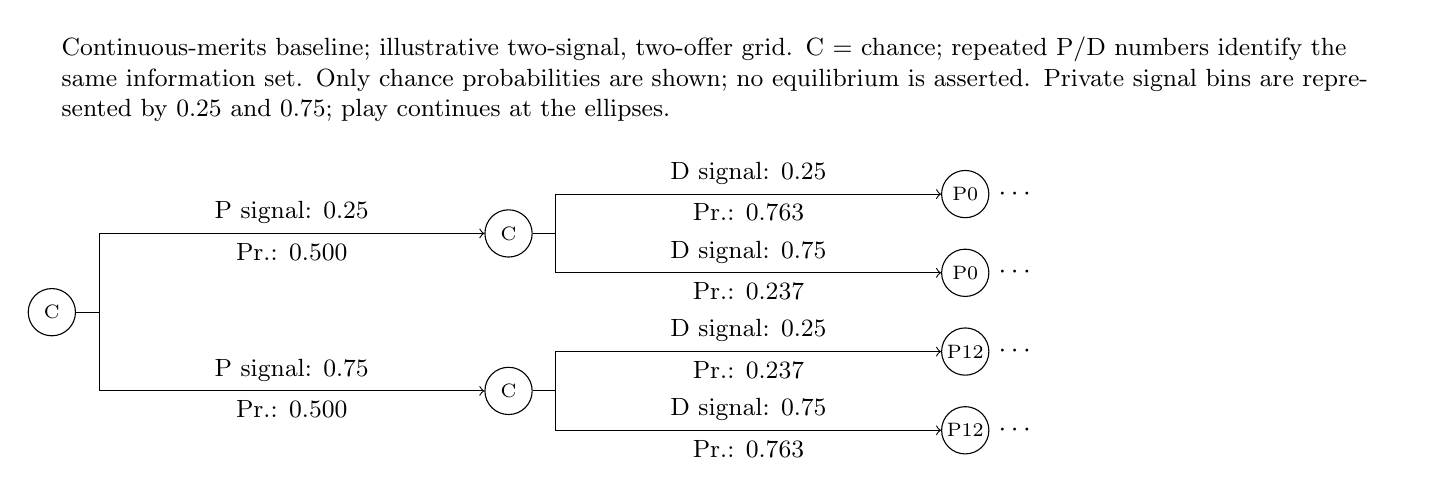
\begin{tikzpicture}
\node[circle, draw, minimum size=0.6cm, inner sep=0pt, font=\scriptsize] (N0) at (0, -1.5) {C};
\node[circle, draw, minimum size=0.6cm, inner sep=0pt, font=\scriptsize] (N1) at (5.8, -0.5) {C};
\node[circle, draw, minimum size=0.6cm, inner sep=0pt, font=\scriptsize] (N2) at (11.6, 0) {P0};
\node[anchor=west] at (11.9, 0) {$\cdots$};
\node[circle, draw, minimum size=0.6cm, inner sep=0pt, font=\scriptsize] (N3) at (11.6, -1) {P0};
\node[anchor=west] at (11.9, -1) {$\cdots$};
\node[circle, draw, minimum size=0.6cm, inner sep=0pt, font=\scriptsize] (N4) at (5.8, -2.5) {C};
\node[circle, draw, minimum size=0.6cm, inner sep=0pt, font=\scriptsize] (N5) at (11.6, -2) {P12};
\node[anchor=west] at (11.9, -2) {$\cdots$};
\node[circle, draw, minimum size=0.6cm, inner sep=0pt, font=\scriptsize] (N6) at (11.6, -3) {P12};
\node[anchor=west] at (11.9, -3) {$\cdots$};
\draw[->] (N0.east) -- (0.6, -1.5) -- (0.6, -0.5) -- (N1.west) node[midway, above, font=\small] {P signal: 0.25} node[midway, below, font=\small] {Pr.: 0.500};
\draw[->] (N0.east) -- (0.6, -1.5) -- (0.6, -2.5) -- (N4.west) node[midway, above, font=\small] {P signal: 0.75} node[midway, below, font=\small] {Pr.: 0.500};
\draw[->] (N1.east) -- (6.4, -0.5) -- (6.4, 0) -- (N2.west) node[midway, above, font=\small] {D signal: 0.25} node[midway, below, font=\small] {Pr.: 0.763};
\draw[->] (N1.east) -- (6.4, -0.5) -- (6.4, -1) -- (N3.west) node[midway, above, font=\small] {D signal: 0.75} node[midway, below, font=\small] {Pr.: 0.237};
\draw[->] (N4.east) -- (6.4, -2.5) -- (6.4, -2) -- (N5.west) node[midway, above, font=\small] {D signal: 0.25} node[midway, below, font=\small] {Pr.: 0.237};
\draw[->] (N4.east) -- (6.4, -2.5) -- (6.4, -3) -- (N6.west) node[midway, above, font=\small] {D signal: 0.75} node[midway, below, font=\small] {Pr.: 0.763};
\node[anchor=south west, align=left, text width=17cm, font=\small] at (0, 0.8) {Continuous-merits baseline; illustrative two-signal, two-offer grid. C = chance; repeated P/D numbers identify the same information set. Only chance probabilities are shown; no equilibrium is asserted. Private signal bins are represented by 0.25 and 0.75; play continues at the ellipses.};

\end{tikzpicture}
\end{document}